\begin{pastexam}[label={px:df3-100-ds-05}]{地方三等資訊處理 100 年 第五題}
（申論；20 分）

給一個加權連通無向圖（weighted connected graph），所有邊線的加權值為正整數。使用下列的貪婪演算法
（Greedy algorithm）尋找從出發的節點 \textit{Start} 到目的地節點 \textit{Goal} 之最短路徑。
\begin{enumerate}[nosep]
\item 初始化集合 \textit{Path} =\{\textit{Start}\}
\item 初始化集合 \textit{VisitedVertices} =\{\textit{Start}\}
\item 如果 \textit{Start} =\textit{Goal}, 離開;否則,繼續第 4 步驟
\item 找出具有最小加權值的邊線 edge（\textit{Start, v}）其中 \textit{v} 不在集合 \textit{VisitedVertices} 內
\item 將 \{\textit{v}\} 加入集合 \textit{Path}
\item 將 \{\textit{v}\} 加入集合 \textit{VisitedVertices}
\item 將 \textit{Start} 設為 \textit{v} 並執行第 3 步驟
\end{enumerate}
\begin{itemize}[leftmargin=2.2em, nosep]
\item[㈠] 請問是否可以正確找到最短路徑？（10 分）
\item[㈡] 請說明原因或理由。（需舉圖例說明理由，否則不予計分）（10 分）
\end{itemize}
\end{pastexam}

\begin{pastsoln}
答案：㈠ 不能。 ㈡ 這個方法每一步只挑「從目前所在的點出去最便宜的邊」，只看眼前一步，不管這條邊通往哪裡、
後面還要走多遠；下面兩個圖例分別說明它會找到比較長的路，甚至走進死路找不到路。

\textbf{反例一：找到的路不是最短。} 下圖 $S$ 是 \textit{Start}，$G$ 是 \textit{Goal}。
\begin{center}
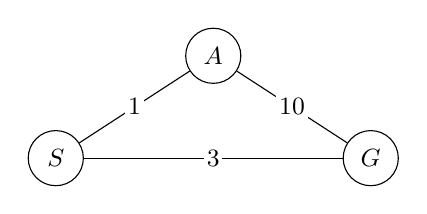
\begin{tikzpicture}[v/.style={circle,draw,minimum size=7mm,inner sep=0pt,font=\small},
  w/.style={font=\small,fill=white,inner sep=1pt}]
\node[v] (S) at (0,0) {$S$};
\node[v] (A) at (2,1.3) {$A$};
\node[v] (G) at (4,0) {$G$};
\draw (S) -- node[w] {1} (A);
\draw (A) -- node[w] {10} (G);
\draw (S) -- node[w] {3} (G);
\end{tikzpicture}
\end{center}
\begin{itemize}
\item 開始：$\mathit{Path} = \{S\}$，目前在 $S$。 $S$ 出去的邊 $(S, A) = 1$、$(S, G) = 3$，挑最小的 $(S, A)$，
走到 $A$。
\item 在 $A$：沒走過的鄰居只有 $G$，走 $(A, G) = 10$ 到 $G$，結束。
\end{itemize}
得到的路是 $S \to A \to G$，長度 $1 + 10 = 11$；真正的最短路徑是直接走 $S \to G$，長度 $3$。

\textbf{反例二：走進死路，根本到不了 Goal。}
\begin{center}
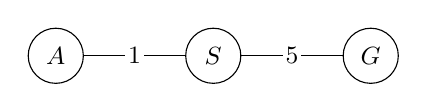
\begin{tikzpicture}[v/.style={circle,draw,minimum size=7mm,inner sep=0pt,font=\small},
  w/.style={font=\small,fill=white,inner sep=1pt}]
\node[v] (A) at (-2,0) {$A$};
\node[v] (S) at (0,0) {$S$};
\node[v] (G) at (2,0) {$G$};
\draw (A) -- node[w] {1} (S);
\draw (S) -- node[w] {5} (G);
\end{tikzpicture}
\end{center}
在 $S$ 挑最小的邊 $(S, A) = 1$ 走到 $A$。 $A$ 唯一的鄰居 $S$ 已經走過，第 4 步找不到邊，演算法卡住（或
沒有定義下一步），永遠到不了 $G$，雖然 $S \to G$ 的路明明存在。

\textbf{為什麼會錯。} 最短路徑要比較的是「從 \textit{Start} 出發的整條路的總長」，這個方法比較的卻是「最後一條
邊的長度」。 便宜的第一步可能接著很貴的後續（反例一），也可能根本不通（反例二）；而且它只沿著一條路往前走、
從不回頭比較別的路。 正確的貪心做法是 Dijkstra 演算法（資結書第~25.3~節）：維護每個點目前已知從起點出發的
最短距離，每次挑「總距離」最小、還沒確定的點，並用它更新鄰居的距離。 在反例一，Dijkstra 會先確定
$d(A) = 1$，但 $d(G) = \min(3, 1 + 10) = 3$，正確得到 $S \to G$。 題目的方法比較像旅行推銷員問題的
「最近鄰居法」，那裡也只是近似，不保證最佳。
\end{pastsoln}
